%!TEX root = ../sbc-template.tex

\subsection{\emph{Smart} TVs}
%!TEX root = ../sbc-template.tex

\emph{Smart} TV é tida como um aparelho de televisão com capacidades interativas ligadas à internet, como aplicativos disponíveis em lojas; acesso a conteúdo online como notícias, previsão do tempo, informações de mercados de ações, mapas e jogos; \emph{e-commerce}; navegação web e acesso a redes sociais\cite{shin2013smart}. Estes aparelhos podem ser equipadas com câmeras e microfones embutidos\cite{michele2014watch}, além de óculos 3D \cite{perakakis2015proposed}, como mostra a Figura \ref{fig:smart_samsung}. Estas televisões utilizam os mesmos sistemas operacionais e conjuntos de aplicativos que computadores comuns, o que as torna sucetíveis às mesmas falhas e ataques de segurança que outros dispositivos semelhates \cite{michele2014watch}.
\begin{figure}
	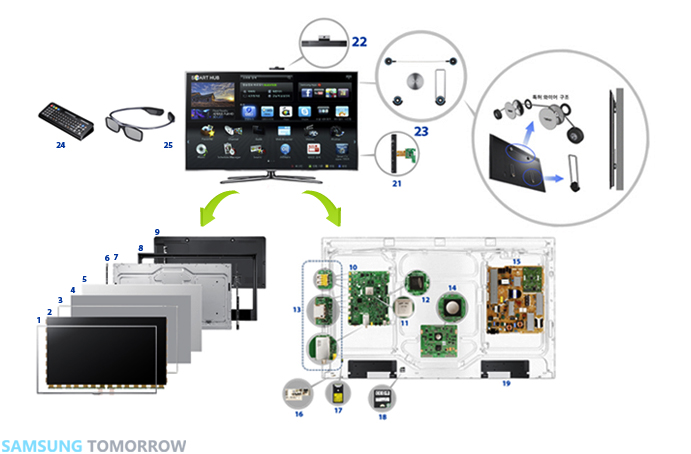
\includegraphics[width=\textwidth]{img/smart_samsung.jpg}
	\caption{\emph{Smart} TV Samsung}
	\label{fig:smart_samsung}
\end{figure}


\subsection{Classificação Indicativa para Conteúdo Televisivo}
%!TEX root = ../sbc-template.tex

O processo de classificação indicativa integra o sistema de garantias dos direitos da criança e do adolescente quanto a promover, defender e garantir o acesso a espetáculos e diversões públicas adequados à condição de seu desenvolvimento, mas reserva-se o direito final aos pais e responsáveis quanto à escolha do conteúdo adequado a estes\cite{eca}.

No Brasil, a \emph{Coordenação de Classificação Indicativa} (Cocind), vinculada ao Ministério da Justiça, é o órgão responsável pela classificação indicativa de obras destinadas à televisão e outros meios, incluindo até mesmo aplicativos. A análise da classificação indicativa realizada pelo Cocind considera o grau de incidência de conteúdos de sexo e nudez, violência e drogas nas obras a serem avaliadas, como sintetizado na Tabela \ref{tab:categorias}. O processo envolve o exame do conteúdo das obras a serem classificadas, a atribuição de classificação indicativa, verificação do cumprimento das normas associadas e advertência por descumprimento destas normas \cite{portaria:ci}.


%!TEX root = ../../novoIndex.tex
\begin{table}[!ht]
  \scalefont{0.8}
  \caption{Categorias de classificação indicativa propostas pela Portaria No. 368, de 11 de Fevereiro de 2014. Fonte: \cite{ci:guia}}
  \label{tab:categorias}
	\centering
	\begin{tabular}{p{4cm} p{1.5cm} p{8cm}}
		\hline
		\textbf{Categoria} & \textbf{Símbolo} & \textbf{Descrição do Conteúdo} \\
		\hline
		Livre & \vfill
\includegraphics[width=0.05\textwidth]{img/livre.png} \vfill&
				Conteúdo predominantemente positivo ou que contem imagens de violência fantasiosa, armas sem violência, mortes sem violência, ossadas e esqueletos sem violência, nudez não erótica e consumo moderado ou inusitado de drogas lícitas. \\
		\hline
		Não recomendado para menores de dez anos &\vfill 
\includegraphics[width=0.05\textwidth]{img/10anos.png}\vfill &
		 		Presença de armas com violência; medo ou tensão; angústia; ossadas e esqueletos com resquícios de ato de violência; atos criminosos sem violência; linguagem depreciativa; conteúdos educativos sobre sexo; descrições verbais do consumo de drogas lícitas; discussão sobre o tráfico de drogas; e o uso medicinal de drogas ilícitas.\\
		\hline
		Não recomendado para menores de doze anos &\vfill 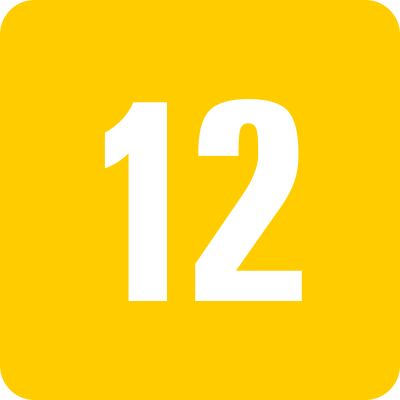
\includegraphics[width=0.05\textwidth]{img/12anos.png}\vfill &
				Ato violento; lesão corporal; descrição de violência; presença de sangue; sofrimento da vítima; morte natural ou acidental com violência; ato violento contra animais; exposição ao perigo; exposição de pessoas em situações constrangedoras ou degradantes; agressão verbal; obscenidade; \emph{bullying}; exposição de cadáver; assédio sexual; supervalorização de beleza física; supervalorização do consumo; nudez velada; insinuação sexual; carícias sexuais; masturbação não explícita; linguagem chula; linguagem de conteúdo sexual; simulações de sexo; apelo sexual; consumo de drogas lícitas; indução ao uso de drogas lícitas; consumo irregular de medicamentos; menção a drogas ilícitas.\\
		\hline
		Não recomendado para menores de catorze anos &\vfill 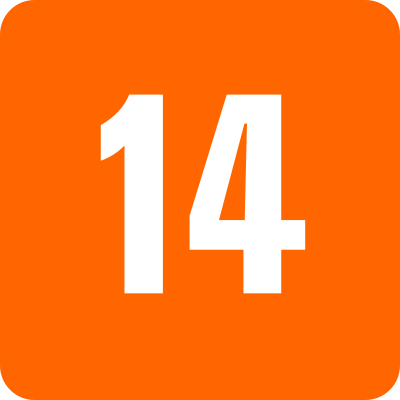
\includegraphics[width=0.05\textwidth]{img/14anos.png}\vfill &
				Morte intencional; estigma ou preconceito; nudez; erotização; vulgaridade; relação sexual não explícita; prostituição; insinuação do consumo de drogas ilícitas; descrições verbais do 	consumo de drogas ilícitas; e discussão sobre a descriminalização de drogas ilícitas.\\
		\hline
		Não recomendado para menores de dezesseis anos &\vfill 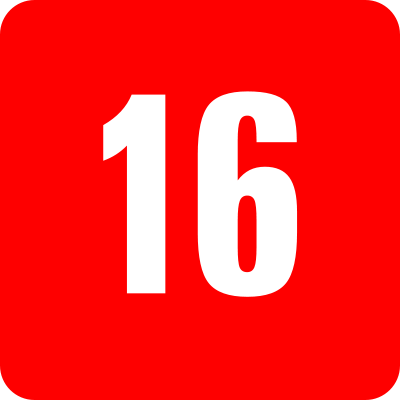
\includegraphics[width=0.05\textwidth]{img/16anos.png}\vfill &
				Estupro; exploração sexual; coação sexual; tortura; mutilação; suicídio; violência gratuita ou banalização da violência aborto, pena de morte ou eutanásia; relação sexual intensa não explícita; produção ou tráfico de qualquer droga ilícita, consumo de drogas ilícitas; indução ao consumo de drogas ilícitas.\\
		\hline
		Não recomendado para menores de dezoito anos &\vfill 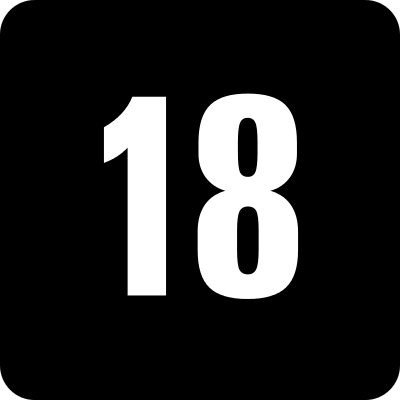
\includegraphics[width=0.05\textwidth]{img/18anos.png}\vfill &
				Violência de forte impacto; elogio, glamourização e/ou apologia à violência; crueldade; crimes de ódio; pedofilia; sexo explícito; situações sexuais complexas ou de forte impacto; apologia ao uso de drogas ilícitas.\\
		\hline
	\end{tabular}
\end{table}


No mundo, conteúdos televisivos são comumente classificados quanto ao grau de incidência de assuntos como linguagem vulgar, conteúdo sexual, drogas e violências, além de temas como conteúdo perturbador e discriminação, a exemplo dos Países Baixos. É frequente a aplicação de restrições de horários para a transmissão de conteúdos restritivos. As classes podem incluir restrição de idade e/ou supervisão de responsáveis, como ocorre nos Estados Unidos, Chile, Equador, Hong Kong, entre outros. Em países como a Austrália e Nova Zelândia, há um sistema de classificação indicativa para televisão aberta e outro para fechada, e um sistema de classificação especial para programas direcionados ao público infantil, na Austrália. Na Colômbia, é proibida a transmissão aérea de pornografia, mesmo em canais adultos. O ícone da classificação indicativa frequentemente deve ser exibido antes do início do programa, antes do início de cada bloco, a exemplo do Brasil, ou durante toda a transmissão do programa, como é o caso da França.  Na Alemanha, apenas o aviso ``O programa a seguir não é recomendado para espectadores abaixo de 16/18 anos'' é mostrado na tela caso haja conteúdo potencialmente ofensivo. Em países como Portugal, Polônia e Singapura, a implantação de sistemas de classificação indicativa é recente, posterior ao ano 2000. \todo{Falta referência}


\subsection{Aprendizagem de Máquina}
Aprendizado de máquina trata de criar modelos que se modificam ou adaptam suas ações para que elas se tornem mais acuradas, enquanto acurácia é medida através do quão bem as ações escolhidas refletem nas corretas.
Um algoritmo que realiza aprendizado de máquina é aquele capaz de aprender a partir de dados, ou experiência, assim como humanos e outros animais. Estes, ao se depararem com determinada, costumam tentar lembrar-se se da última vez em que estiveram em uma situação parecida, tentaram alguma ação que pode ter dado certo -- então deve ser repetida-- ou errado -- então deve tentar algo diferente --adaptação \cite{marsland2015machine}, \cite{goodfellow2016deep}. De acordo com a definição clássica de \cite{mitchell1997machine}, um algoritmo que aprende a partir da experiência $E$ quanto a um conjunto de tarefas $T$ e medida de performance $P$, se sua performance nas tarefas em $T$, medida por $P$, melhora com a experiência $E$.
Algumas tarefas que podem ser atacadas utilizando aprensdizado de máquina são a classificação, regressão, transcrição, tradução automática, detecção de anomalia, síntese e amostragem \cite{goodfellow2016deep}.

\subsection{\emph{Deep Learning}}
Aprendizagem profunda é um conjunto de técnicas de aprendizagem de máquina que se baseiam em modelos com arquiteturas profundas, compostas de vários níveis de operações não lineares, a exemplo das redes neurais com múltiplas camadas escondidas ou um conjunto de fórmulas proposicionais que re-utiliza várias sub-fórmulas \cite{bengio2009learning}. Estes modelos ganharam popularidade com o aumento da quantidade de dados disponíveis sobre temas complexos, aliado com o aumento da disponibilidade de recursos computacionais para executar modelos mais robustos e o aumento de tamanho dos conjuntos de dados disponíveis \cite{goodfellow2016deep}. De acordo com a IBM, são gerados $2,5$ quintilhões de bytes de dados por dia, e $90\%$ do volume de dados presente no mundo hoje foi criado nos últimos dois anos \cite{ibm2017bigdata}.


\subsection{Redes Neurais Convolucionais}
Redes neurais convolucionais (RNC) são um tipo de rede neural específico para o processamento de dados que têm uma topologia bem definida e estruturada em uma grade, a exemplo de séries temporais e imagens. Sua principal característica envolve o uso de convoluções no lugar de multiplicações de matrizes em ao menos uma das camadas da rede neural.\cite{goodfellow2016deep}.

Cada camada das redes neurais convolucionais é composta por uma etapa de convolução, seguida por uma ativação não-linear, finalizando em \emph{pooling}, como mostra a Figura \ref{fig:cnn_camada}. A seguir, serão explanadas cada uma destas etapas.

\begin{figure}
	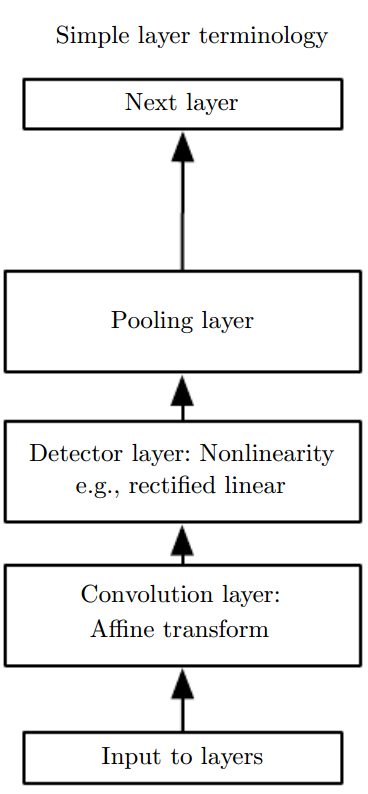
\includegraphics[height=0.5\textheight]{img/cnn_camada.png}
	\caption{Componentes de uma camada de uma rede neural convolucional \cite{goodfellow2016deep}. }
	\label{fig:cnn_camada}
\end{figure}

\subsubsection{Convolução}
A operação de convolução descreve a média ponderada de uma determinada função $x_1(t)$ sob um intervalo fixo de uma variável, enquanto os pesos da média ponderada considerada pertencem à função $x_2(t)$ amostrados em intervalos $a$ \cite{bracewell1986fourier}. Assim, a convolução $s(t)$ de duas funções $x_1(t)$ e $x_2(t)$ é uma função $f: \mathds{Z} \rightarrow \mathds{R}$ representada simbolicamente por $x_1(t) * x_2(t)$ e definida de acordo com a Equação \ref{eq:int_convolucao} \cite{lathi2006sinais}.
\begin{equation}\label{eq:int_convolucao}
	s(t) = x_1(t) * x_2(t) = \int_{-\infty}^{\infty} x_1(a) x_2(t-a)da
\end{equation}

Quando a operação de convolução é aplicada em aprendizagem de máquina, a primeira função $x_1(t)$ é chamada de \emph{input (entrada?)}, a segunda função $x_2(t)$ é chamada de \emph{kernel (núcleo?)}, e a saída $s(t)$ é chamada de mapa de \emph{feature map (mapa de características?)}. Neste caso, a entrada normalmente é um vetor multidimensional de dados e o núcleo é um vetor multidimensional de pesos que devem ser adaptados pelo algoritmo de aprendizado de máquina. Em redes neurais convolucionais, os vetores multidimensionais de entrada e núcleo são chamados tensores. Além disto, assume-se que os valores dos tensores são zero em todos os pontos menos os que estão guardados em memória, ou seja, a operação de convolução é implementada apenas nas posições declaradas dos vetores de dados e peso. Assim, para uma imagem bidimensional de tamanho $(m,n)$ $I$ como entrada, tem-se um núcleo bidimensional $K$, e a operação de convolução é definida como exemplificado na Equação \ref{eq:conv_img}, para cada posição $(i,j)$ do mapa de características resultante \cite{goodfellow2016deep}.

\begin{equation}\label{eq:conv_img}
	S(i,j) = I(i,j)*K(i,j) = \sum_{m}\sum_{n}I(m,n)K(i-m,j-n)
\end{equation}

A convolução é comutativa, ou seja, as Equações \ref{eq:conv_img_eq} e \ref{eq:conv_img} são equivalentes, salvo que no primeiro caso há a convolução da imagem pelo núcleo, enquanto no segundo há a convolução do núcleo pela imagem. Comumente, a Equação \ref{eq:conv_img} é a implementada em algoritmos de redes neurais convolucionais, haja visto que existem menor variação no intervalo de valores válidos de $m$ e $n$, o que diminui o custo computacional.

\begin{equation}\label{eq:conv_img_eq}
	S(i,j) = K(i,j)*I(i,j) = \sum_{m}\sum_{n}I(i-m,j-n)K(m,n)
\end{equation}

A propriedade comutativa surge graças à ação de revolver o núcleo em relação à imagem, e não tem aplicação prática. Porém, esta propriedade não tem fins práticos além da prova da operação de convolução. Assim, é comum que seja implementada correlação cruzada, indicada na Equação \ref{eq:correlacao_img_eq}, semelhante à convolução dada na Equação \ref{eq:conv_img_eq} sem que haja o espelhamento do núcleo em relação à imagem.

\begin{equation}\label{eq:correlacao_img_eq}
	S(i,j) = I(i,j)*K(i,j) = \sum_{m}\sum_{n}I(i+m,j+n)K(m,n)
\end{equation}

\subsubsection{Pooling}

Depois de realizar várias operações de convolução em paralelo para gerar um conjunto de ativações lineares e alimentá-las a funções de ativação não-lineares, como \emph{ReLU}, \emph{Softmax}, etc, na chamada etapa de detecção, chega-se à etapa de \emph{pooling}. Uma função de \emph{pooling} substitui a saída da rede em determinada localização por uma síntese estatística das saídas vizinhas. Por exemplo, a função \emph{max pooling} retorna o valor máximo em uma área retangular, enquanto a \emph{average pooling} retorna a média das saídas de um retângulo. O objetivo destas funções é fazer com que


\subsection{Modelos clássicos de Redes Neurais Convolucionais}
Estes modelos trouxeram grandes inovações quanto à arquitetura das redes neurais convolucionais.
\subsubsection{LeNet}

\subsubsection{AlexNet}

\subsubsection{GoogleLeNet ou Inception}

\subsubsection{ResNet}

\subsubsection{SSD}

\subsubsection{YOLO}
